\chapter{Brief Introduction to Calculus of Variations} \label{ch:calculusofvariations}

Calculus of variations studies the change of the value of a functional w.r.t the choice of function. A commonly seen objective of calculus of variations is to find the optimal function among a set of functions (usually defined by restrictions) that maximizes or minimizes a functional.

Notice that under the scope of this notebook, only a few ideas from calculus of variations are needed. Therefore, only a brief introduction is introduced. More details about calculus of variations can be found in another notebook \textit{A Notebook on Calculus}.

\section{Problem Formulation}

Consider a cost function defined by
\begin{eqnarray}
	J &=& \int_{0}^{T} h\left(x(t), t\right)dt \label{eq:calculusofvariations:problem}
\end{eqnarray}
where $x(t)$ is a function of $t$. The objective is to find $x(t)$ in the searching space that minimizes the above cost function. 

\section{Brief Discussion of the Solution}

Similar with static optimization, the solution to \eqref{eq:calculusofvariations:problem} can be obtained by studying how the change of each element in the cost function would affect the change of the value of the cost function, i.e., how $dx(t)$ and $dt$ affect $dJ$.

There are some obvious differences of \eqref{eq:calculusofvariations:problem} comparing with discrete time optimization such as the following
\begin{eqnarray}
	J &=& \sum_{k=0}^{N-1} h\left(x(k), u(k)\right) \label{eq:calculusofvariations:problem2}
\end{eqnarray}
The major differences are
\begin{enumerate}
	\item In \eqref{eq:calculusofvariations:problem} integration is used, while in \eqref{eq:calculusofvariations:problem2} sum is used.
	\item In \eqref{eq:calculusofvariations:problem}, the two variables $x(t)$ and $t$ are correlated, while in \eqref{eq:calculusofvariations:problem2}, $x(t)$ and $u(t)$ can be treated as independent variables, with the system dynamics $x(k+1) = f\left(x(k) + u(k)\right)$ the equality constraint.
\end{enumerate}
Integration and sum are in the essence describing the same thing, where integration a limiting case of sum. Therefore, this first difference does not affect much how we would proceed with the calculation. It is the second difference that forms the main challenge.

Consider $x(t)$ being a function of $t$ defined from $t=0$ to $t=T$. Consider a neighborhood function $x(t) + dx(t)$. Notice that the neighborhood function $x(t) + dx(t)$ is not necessarily cut-off at $t=T$. Without loosing generality, assume that the neighborhood function is stretched from $t=T$ to $t=T+dT$. The final value of the original and the neighborhood functions can be bridged as follows.
\begin{eqnarray}
	\left.\left[x(t) + dx(t)\right]\right|_{t=T+dT} - x(T) &=& \delta x(T) + \dot{x}(T)dT \nonumber
\end{eqnarray}
where $\delta x(T)$ describes a portion of the final value increment of the neighborhood function irrelevant to change in time, and $\dot{x}(T)dT$ the portion caused due to the change in time. Notice that since $x(t)$ and $x(t)+dx(t)$ are close enough, their slope at $t=T$ shall be approximately the same. This is demonstrated by Fig. \ref{fig:calculusofvariations:calculus_of_variations}.

\begin{figure}
	\centering
	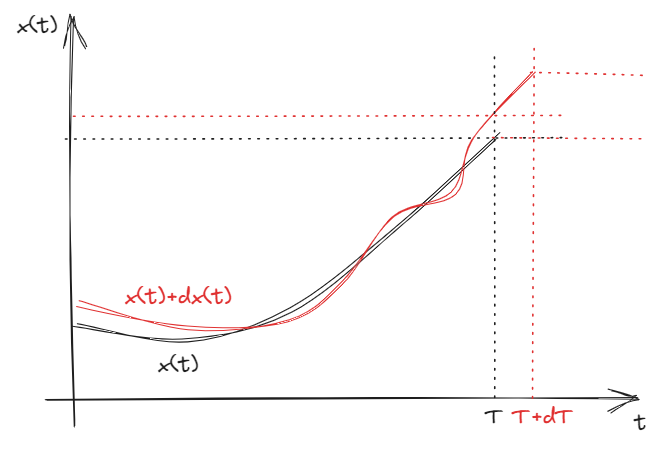
\includegraphics[width=250pt]{chapters/ch-optimal-robust-control-system/figures/calculus_of_variations.png}
	\caption{A demonstration of the calculation of $dx(T)$ from calculus of variations perspective.}
	\label{fig:calculusofvariations:calculus_of_variations}
\end{figure}

Another relation that describes $dJ$ in \eqref{eq:calculusofvariations:problem} is given below. This is known as the Leibniz's rule for functionals.
\begin{eqnarray}
	dJ &=& h\left(x(T), T\right)dT - h\left(x(0), 0\right)dt_0 + \int_{t=0}^{T}\left(h_x^T\left(x(t), t\right)\delta x(t)\right)dt \nonumber
 \end{eqnarray}
where $dT$ and $dt_0$ describe the stretch of the neighborhood function at the end and the beginning w.r.t. $t$, respectively, and 
\begin{eqnarray}
	h_x &=& \dfrac{\partial h}{\partial x} \nonumber
\end{eqnarray} 






